
\section{ Linear regression }
\subsection{Stochastic gradient descendent}


Stochastic gradient descendent (SGD) is a sequential version of the gradient descent. Instead of considering the full batch gradient on all $N$
training data points, we consider a stochastic version of the gradient. First, pick a training data point $(x_n, y_n)$ uniformly random
(hence the name 'stochastic') and consider only the error on that data point.  \cite{LFD}

The gradient of this single data point's error is used for the weight update in exactly the same that the gradient was used in batch gradient descent.

Another variants are the \textbf{mini-batch gradient descent} and the \textbf{batch gradient descendent}, the differences among them are the size of the batch: one for the pure stochastic gradient descendent, between 32 or 64 for the mini-batch variation and more than that for the batch gradient descendent.


\subsection{Pseudo - inverse algorithm}
Pseudo inverse algorithm also known as \textbf{linear regression algorithm} or \textbf{ordinary least squares}(OLS) is based on minimizing the squared error between the 
projection matrix $h(x) = w^T x$ and $y$, the target vector, where $x \in \mathbb R^{N \times (d+1)}$ is the feature matrix and
$N \in \mathbb N$ the training data size.   

\begin{equation*}
  E_{in}(w) = \frac{1}{N} \sum_{n=1}{N} (w^T x_n - y)^2 
  = \frac{1}{N} \| Xw -y \|^2 
\end{equation*}

Where $\|.\|$ is the Euclidean norm of a vector.

Since $E_{in}(w)$ is differentiable we can use standard matrix calculus to find the $w$ that minimizes  $E_{in}$ with respect to w:

$$\nabla E_{in}(w) = \frac{2}{N}(X^TXw - X^T y) =0$$
Finally to get $\nabla  E_{in}(w)$ to be $0$, we should find a $w$ that satisfies

$$X^TXw = X y$$

If $X^TX$ is invertible, $w = X^\dagger y$ where $X^\dagger = (X^T X)^{-1}$ is the \texttt{pseudo-inverse} of $X$. The resulted $w$ is the unique optimal solution that minimizes $E_{in}$.  Otherwise a pseudo-inverse can still be defined, but the solution will not be unique.

In practice, $X^TX$ is invertible in most of the cases since $N$ is often much more bigger than $d+1$, so there will likely be $d+1$ linearly independent vector $x_n$.



\subsection{Exercise 1}

Estimate a linear regression model from the data provided by the
feature vectors (Average intensity, Symmetry)
using both the pseudo-inverse algorithm and the Stochastic Gradient Descent (SGD).
The labels will be $\{-1,1\}$,
one for each feature vector of each number.
Draw the solutions obtained together with the data used in the fitting.
Assess the goodness of the result using $E_{in}$ and $E_{out}$
(for Eout calculate the predictions using the data from the test file).



\subsubsection{Error}


As we have said the error is the mean squared error:
$$E_{out}(h) = \mathbb E [(h(x) -y)^2]$$
 $$E_{in}(w)  = \frac{1}{N} \| Xw -y \|^2$$

A direct implementation is

\begin{minted}{python}
  def Error(x,y,w):
    '''quadratic error 
    INPUT
    x: input data matrix
    y: target vector
    w:  vector to 

    OUTPUT
    quadratic error >= 0
    '''
    error_times_n = np.linalg.norm(x.dot(w) - y.reshape(-1,1))**2
  
    return error_times_n/len(x)

  \end{minted}

  

  For the euclidean norm we have used \texttt{np.linalg.norm} \cite{norm} numpy function.

  The gradient computation is direct too:

  $$\nabla E_{in}(w) = \frac{2}{N}(X^TXw - X^T y)= \frac{2}{N}(X^T(Xw -  y))$$
  
\begin{minted}{python}
  def dError(x,y,w):
  ''' gradient
  OUTPUT
  column vector
    '''

    return (2/len(x)*(x.T.dot(x.dot(w) - y.reshape(-1,1))))
  \end{minted}

  \subsubsection{Interpretation of the mean squared error, E}
  The mean squared error function $E: \mathbb R ^d \longrightarrow \mathbb R^+_0$ measures the average of the squared difference between the estimated values and the actual value\cite{MSE}. Hence, the nearer to zero, the better.

  
  

\subsubsection{Pseudo-inverse algorithm}

As we have described in pseudo inverse introduction, firstly we need to compute the pseudo-inverse. For that we have use  \texttt{np.linalg.pinv} \cite{pseudo-inverse}function from numpy library.

\begin{minted}{python}
  def pseudoInverseMatrix ( X ):
    '''
    INPUT 
    X: is a matrix (must be a np.array) to use transpose and dot method
    OUTPUT
    hat matrix 
    '''

    '''
    #S =( X^TX ) ^{-1}
    simetric_inverse = np.linalg.inv( X.T.dot(X) )

    # S X^T = ( X^TX ) ^{-1} X^T
    return simetric_inverse.dot(X.T)
    '''
    return np.linalg.pinv(X)
\end{minted}

Finally we have to compute $w = X^\dagger y$


\begin{minted}{python}
  def pseudoInverse(X, Y):
    ''' 
    INPUT
    X is the feature matrix 
    Y is the target vector (y_1, ..., y_m)
    
    OUTPUT: 
    w: weight vector
    '''
    X_pseudo_inverse = pseudoInverseMatrix ( X )
    Y_transposed = Y.reshape(-1, 1)
    
    w = X_pseudo_inverse.dot( Y_transposed)
    
    return w

  \end{minted}

  \subsubsection{Pseudo-inverse linear regression model}

  After computing the algorithm we obtain:

\begin{verbatim}
___ Goodness of the Pseudo-inverse fit ___

  Ein:   0.07918658628900395
  Eout:  0.1309538372005258

Evaluating output training data set
Input size:  1561
Bad negatives : 7
Bad positives : 3
Accuracy rate : 99.35938500960923 %

Evaluating output test data set
Input size:  424
Bad negatives : 1
Bad positives : 7
Accuracy rate : 98.11320754716981 %

\end{verbatim}

  Which means that the $w$ computed by our pseudo-inverse algorithm by the training data set has a $E_{in}(w) = 0.079$ and by the test data $E_{out}(w) = 0.131$, for our experiment it is a good fit, because it is closed enough to zero. In addition, if we evaluate the data classification,
  from $1561$ training data it only misclassify $10$ points, whereof 7 was truly positives. The accuracy rate $(\frac{\text{good classified data}}{\text{data set size}})$
  is $99.358 \%$, which continues being really good.

  Initially, we could think that it classifies the positives values better, but if we analyse the output from test data set, there are more negatives values misclassified, so we cannot establish any relation. Moreover here the accuracy rate is $98.113 \%$

  Finally, a graphic representation for the solutions is

  
  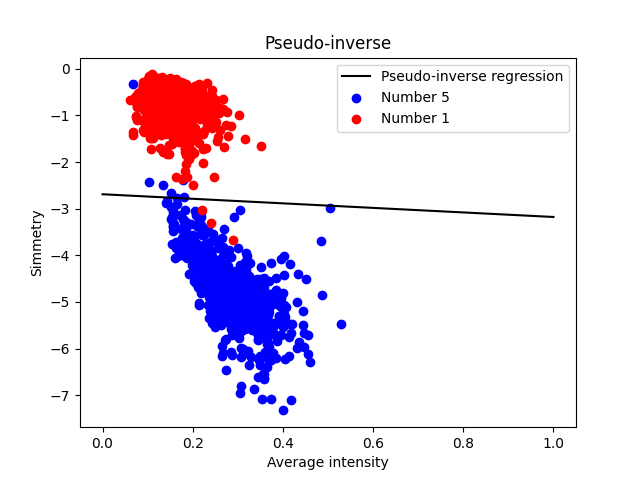
\includegraphics[width=\linewidth]{2_1_pseudo_inverse.png}


  Something really import about this method is that it is equal or better than the gradient descent, therefore in the next experiments
  we are going to compare the results which it. 

  \subsubsection{How have we plotted the regression line.}

  Firstable, to draw a line we need two points.

  Therefore we use the sign um to classify the numbers, we are going to find two points in $\mathbb R^2$ that their estimation is zero, which means that they are in the middle of classification (the regression line).

  The obtained weight vector $w^T = (w_1,w_2,w_3)$, means that for a point $(x,y) \in \mathbb R^2$
  its estimation is $h(x,y) = (1,x,y) w = w_1 + w_2x + w_3y$.

  To calculate the two points we are going to equalize $h(x,y)=0$ and from the infinity solutions we would compute two:

  if $x=0$ then $y = \frac{- w_1}{w_3}$, and if  $x=1$ then $y = \frac{- w_1 - w_2}{w_3}.$
  

  The related code is


  \begin{minted}{python}
    # regression line
    # x= 0
    symmetry_for_cero_intensity = -w[0]/w[2]

    #  x = 1, 0 = w0 + w1 * w2 * x2
    # then y = (-w0 - w1) /w2
    symmetry_for_one_intensity= (-w[0] - w[1])/w[2]

    # plotting order
    plt.plot([0, 1],
             [symmetry_for_cero_intensity,symmetry_for_one_intensity],
             'k-',
             label=(title+ ' regression'))
     
  \end{minted}

  
  \subsubsection{Stochastic gradient descendent}

  Based on the description of the algorithm, we have done two implementations:

  This one is strictly based on the classroom's slides, however depending on the \texttt{batch\_size} the exact number of iterations will be
$$\texttt{max\_iter} \times \lfloor \frac{ \texttt{(len(y))}}{\texttt{ batch\_size}} \rfloor$$ 

  
  \begin{minted}{python}
def sgd(x,y, eta = 0.01, max_iter = 1000, batch_size = 32, error=10**(-10)):
        '''
        Stochastic gradient descent
        INPUT 
        x: data set
        y: target vector
        eta: learning rate
        max_iter 

        OUTPUT 
        w: weight vector
        '''
  
        #initialize data
        w = np.zeros((x.shape[1], 1), np.float64)
        n_iterations = 0

        len_x = len(x)
        x_index = np.arange( len_x )
        batch_start = 0
        w_error = Error(x,y,w)

        while n_iterations < max_iter and w_error > error :
  
                #shuffle and split the same into a sequence of mini-batches
                np.random.shuffle(x_index)
                for batch_start in range(0,  len_x, batch_size):
                        iter_index = x_index[ batch_start : batch_start + batch_size]

        
                        w = w - eta* dError(x[iter_index, :], y[iter_index], w)
        
                n_iterations += 1
                w_error = Error(x,y,w)

   
        return w
      \end{minted}

      In order to control exactly the numbers of iterations we are going to use this function: 

      \begin{minted}{python}
        def sgd_exact_number_iter(x,y, eta = 0.01,
        max_iter = 1000, batch_size = 32, error = 10**(-10)):
        '''
        Stochastic gradient descent
        INPUT 
        x: data set
        y: target vector
        eta: learning rate
        max_iter 
        OUTPUT 
        w: weight vector
        '''
        #initialize data
        w = np.zeros((x.shape[1], 1), np.float64)
    
        n_iterations = 0
        batch_start = 0
        len_x = len(x)
    
        x_index = np.arange( len_x )
        w_error = Error(x,y,w)
 
        while n_iterations < max_iter and w_error > error:
                #shuffle and split the same into a sequence of mini-batches
                if batch_start == 0:
                        x_index = np.random.permutation(x_index)
                iter_index = x_index[ batch_start : batch_start + batch_size]

                w = w - eta* dError(x[iter_index, :], y[iter_index], w)
                
                n_iterations += 1

                batch_start += batch_size
                if batch_start >= len_x: # if end, restart
                        batch_start = 0
                
                w_error = Error(x,y,w)


        return w

      \end{minted}


      Due to the fact that this is a stochastic method and the gradient's descent does not reduce the error in every step,  there are other variations, for example we can save and return only the $w$ found which has the less error.


       \begin{minted}{python}
         def sgd_save_w(x,y, eta = 0.01, max_iter = 1000,
                                   batch_size = 32, error = 10**(-10)):
        '''
        Stochastic gradient descent
        INPUT 
        x: data set
        y: target vector
        eta: learning rate
        max_iter 
        OUTPUT 
        w: weight vector
        '''
        #initialize data
        w = np.zeros((x.shape[1], 1), np.float64)
    
        n_iterations = 0
        batch_start = 0
        len_x = len(x)
    
        x_index = np.arange( len_x )
        w_error = Error(x,y,w)

        #IMPROVEMENT
        best_error = w_error
        best_w = w 
 
        while n_iterations < max_iter and w_error > error:
                #shuffle and split the same into a sequence of mini-batches
                if batch_start == 0:
                        x_index = np.random.permutation(x_index)
                iter_index = x_index[ batch_start : batch_start + batch_size]

                w = w - eta* dError(x[iter_index, :], y[iter_index], w)
                
                n_iterations += 1

                batch_start += batch_size
                if batch_start >= len_x: # if end, restart
                        batch_start = 0
                
                w_error = Error(x,y,w)

                # IMPROVEMENT  
                if w_error < best_error:
                        best_w = w
                        best_error = w_error


        return best_w

      \end{minted}

    This algorithm is interesting because it returns the best $w$ found and has (in order) the same computational cost. 


    \paragraph{Initial point}

    Another consideration is that as we know, it is really important the chosen of the initial point in gradient descendent. However, due to the fact that we are working with the mean quadratic error, we know that only exists  one global minimum, so here the relevance of the initial point is to reduce iterations. Therefore we theoretically do not have more information,  we have chosen the $w_0 = 0 \in \mathbb R^d.$


    \paragraph{The experiment result}  We are going to execute the \texttt{sgd} algorithm (our version)  with $\eta = 0.01$ batch sizes $1,32, 200 \text{ and } \texttt{len(y)}$ and the numbers of steps $50 \text{ and } 300$.


   


\begin{table}[H]
\begin{tabular}{|c|c|c|c|c|c|}
\hline
   Batch size &  Iterations & $E_{in}$      & $E_{out}$                  & Training accuracy rate $(\%)$   & Test accuracy rate $(\%)$   \\ \hline
  1          &     50     &     0.0798    & 0.131                      &        99.423           & 98.349    \\ \hline
 32          &     50     &   0.081       &      0.133                 & 99.295            &   98.113       \\ \hline
200          &         50 &     0.082     &    0.135                   &      99.424          & 98.113       \\ \hline
 1561        & 50         & 0.404         &  0.428                      &   99.167        & 95.28            \\ \hline              
\end{tabular}
\end{table}


As we can see, as bigger is the batch size the worse is the error.
Something really interesting is that we are minimizing based on the quadratic error, but it does not mean we are minimizing the accuracy error ( there is a correlation but not a coincidence. A good example of that is if we compare bath's size 200 with bath's size 32.  
As we increase the numbers of iterations the general error decrease (see 300 steps). 


Another interesting observation is that for batch's size one,   200 iterations is worse than 50, this is because we are oscillating over the solution. The algorithm we have described which saves the best $w$, \texttt{sgd\_save\_w} would solve this problem. 

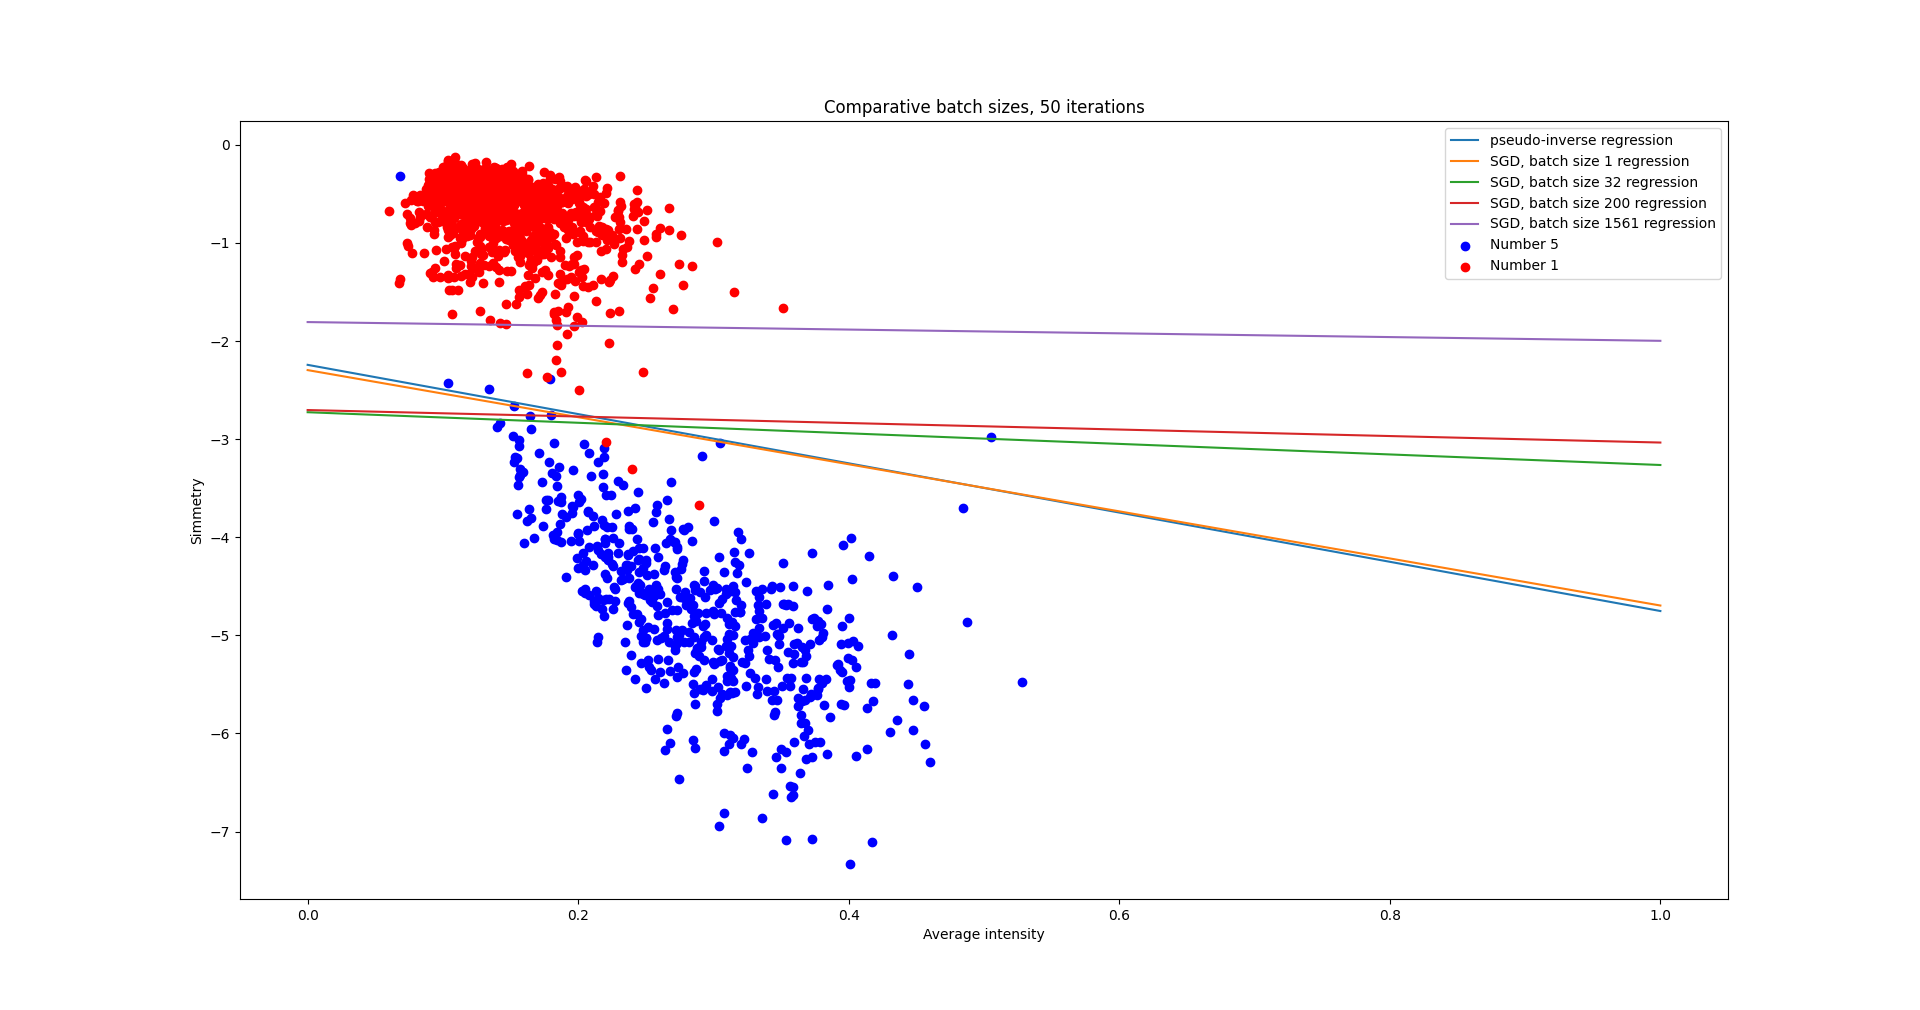
\includegraphics[angle=90,width=\linewidth]{2_1_comparatives_50.png}

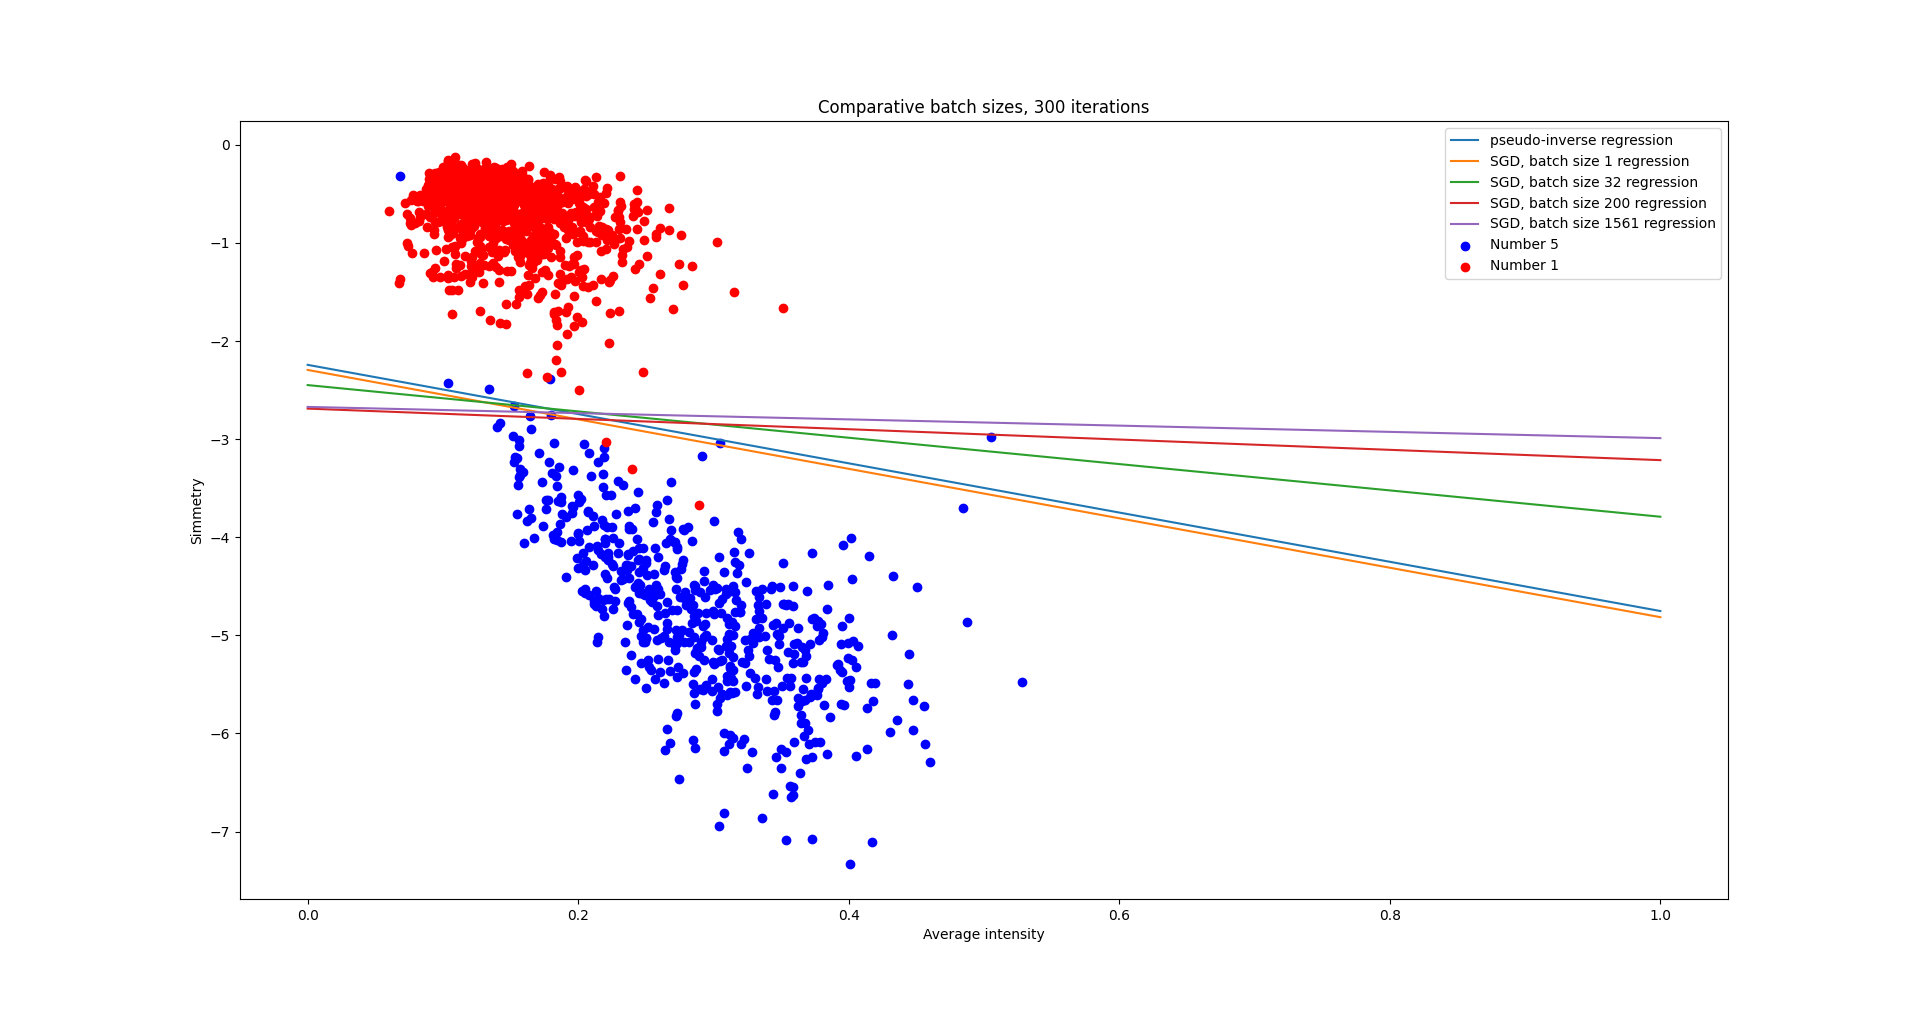
\includegraphics[angle=90,origin=c,width=\linewidth]{2_1_comparatives_300.png}


   \paragraph{50 steps} 
    \begin{verbatim}

___ Goodness of the Stochastic Gradient Descendt (SGD) fit ___


	SGD, batch size 1
Ein:  0.07981803904587495
Eout:  0.13188855705205335

Evaluating output training data set
For w^T = [[-1.15690746 -1.20909308 -0.50379833]]
Input size:  1561
Bad negatives : 6
Bad positives : 3
Accuracy rate : 99.4234465086483 %

Evaluating output test data set
For w^T = [[-1.15690746 -1.20909308 -0.50379833]]
Input size:  424
Bad negatives : 0
Bad positives : 7
Accuracy rate : 98.34905660377359 %

--- End of a section, press any enter to continue ---


	SGD, batch size 32
Ein:  0.08183880846320654
Eout:  0.13300563169544255

Evaluating output training data set
For w^T = [[-1.23840622 -0.24445313 -0.45432575]]
Input size:  1561
Bad negatives : 8
Bad positives : 3
Accuracy rate : 99.29532351057014 %

Evaluating output test data set
For w^T = [[-1.23840622 -0.24445313 -0.45432575]]
Input size:  424
Bad negatives : 1
Bad positives : 7
Accuracy rate : 98.11320754716981 %

--- End of a section, press any enter to continue ---


	SGD, batch size 200
Ein:  0.0824097083428238
Eout:  0.13514678139988967

Evaluating output training data set
For w^T = [[-1.21138905 -0.14846307 -0.44806566]]
Input size:  1561
Bad negatives : 6
Bad positives : 3
Accuracy rate : 99.4234465086483 %

Evaluating output test data set
For w^T = [[-1.21138905 -0.14846307 -0.44806566]]
Input size:  424
Bad negatives : 1
Bad positives : 7
Accuracy rate : 98.11320754716981 %

--- End of a section, press any enter to continue ---


	SGD, batch size 1561
Ein:  0.40484272492435486
Eout:  0.42805781278130317

Evaluating output training data set
For w^T = [[-0.42953442 -0.04548081 -0.23773542]]
Input size:  1561
Bad negatives : 1
Bad positives : 12
Accuracy rate : 99.16720051249199 %

Evaluating output test data set
For w^T = [[-0.42953442 -0.04548081 -0.23773542]]
Input size:  424
Bad negatives : 0
Bad positives : 20
Accuracy rate : 95.28301886792453 %

--- End of a section, press any enter to continue ---

\end{verbatim}

   
      \paragraph{300 steps} 
\begin{verbatim}

	SGD, batch size 1
Ein:  0.07991429824341009
Eout:  0.13043428762931666

Evaluating output training data set
For w^T = [[-1.14204678 -1.25437994 -0.4976879 ]]
Input size:  1561
Bad negatives : 7
Bad positives : 3
Accuracy rate : 99.35938500960923 %

Evaluating output test data set
For w^T = [[-1.14204678 -1.25437994 -0.4976879 ]]
Input size:  424
Bad negatives : 0
Bad positives : 7
Accuracy rate : 98.34905660377359 %

--- End of a section, press any enter to continue ---

	SGD, batch size 32
Ein:  0.08063407701065878
Eout:  0.13581316178349648

Evaluating output training data set
For w^T = [[-1.18587205 -0.6497891  -0.48419008]]
Input size:  1561
Bad negatives : 5
Bad positives : 3
Accuracy rate : 99.48750800768738 %

Evaluating output test data set
For w^T = [[-1.18587205 -0.6497891  -0.48419008]]
Input size:  424
Bad negatives : 0
Bad positives : 7
Accuracy rate : 98.34905660377359 %

--- End of a section, press any enter to continue ---


	SGD, batch size 200
Ein:  0.08138110980377243
Eout:  0.1344240103546277

Evaluating output training data set
For w^T = [[-1.23721465 -0.24176584 -0.46011533]]
Input size:  1561
Bad negatives : 7
Bad positives : 3
Accuracy rate : 99.35938500960923 %

Evaluating output test data set
For w^T = [[-1.23721465 -0.24176584 -0.46011533]]
Input size:  424
Bad negatives : 1
Bad positives : 7
Accuracy rate : 98.11320754716981 %

--- End of a section, press any enter to continue ---


	SGD, batch size 1561
Ein:  0.085568968925448
Eout:  0.13713701679830562

Evaluating output training data set
For w^T = [[-1.15962485 -0.13812568 -0.43405538]]
Input size:  1561
Bad negatives : 5
Bad positives : 3
Accuracy rate : 99.48750800768738 %

Evaluating output test data set
For w^T = [[-1.15962485 -0.13812568 -0.43405538]]
Input size:  424
Bad negatives : 0
Bad positives : 7
Accuracy rate : 98.34905660377359 %

--- End of a section, press any enter to continue ---

\end{verbatim}



\section{Experiment }

\subsection{a) Generate a training sample}

We are going to use a uniform generation:

\begin{minted}{python}
def simula_unif(N, d, size):
        ''' generate a trining sample of N  points
in the square [-size,size]x[-size,size]
'''
        return np.random.uniform(-size,size,(N,d))
 
\end{minted}

After fixed random seed to $1$.

The final 2D map  is

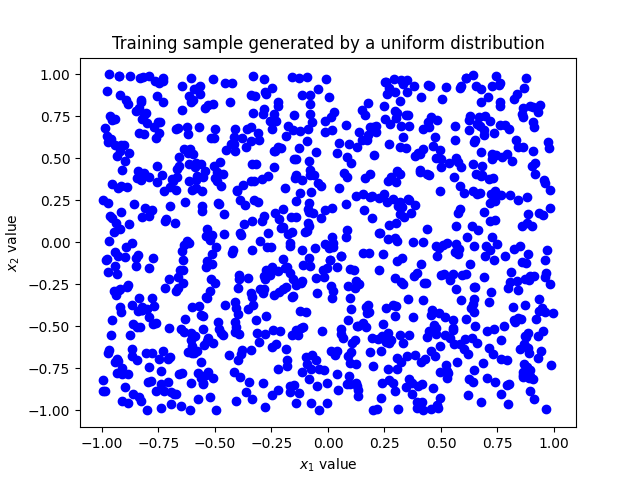
\includegraphics[width=\linewidth]{2_2_a_training_sample.png}

\subsection{b) Labels, noise and map}

b) Let's consider the function $f(x_1, x_2) = sign((x_1 - 0.2)^2 + x_2^2 - 0.6)$ that we will use to assign a label to each point of the previous sample. We introduce noise on the labels, randomly changing the sign of 10 \% of them.
Draw the obtained labels map.


Before plotting, it is important to have in mind that a circumference with radius $r$ and center $(c_1, c_2) \in \mathbb R^2$ are the points $(x_1, x_2) \in \mathbb R^2$ that verify 

\[ (x_1 - c_1)^2 + (x_2 - c_2)^2 = r^2\]

Therefore looking at $f$ it is easy to think that we are going to see a circle of radius $\sqrt{0.6}$ and center $(0.2, 0)$.

The plotting is

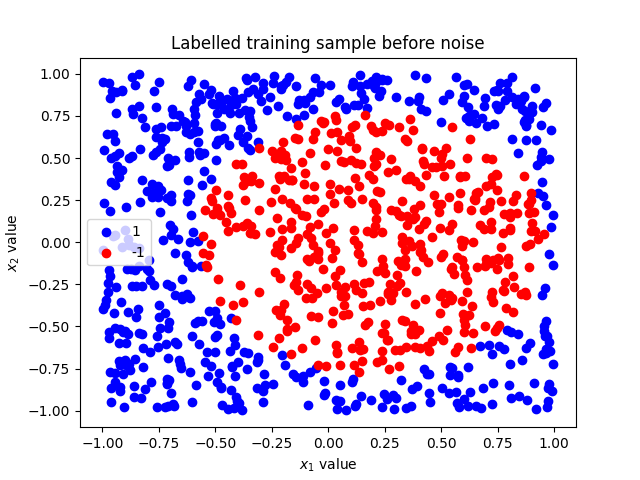
\includegraphics[width=\linewidth]{/2_2_b_labelled_before_noise.png}

In order to introduce noise on the label we are going to change randomly the sign of the $10\%$ of  the labels obtained by $b$.



\begin{minted}{python}
#labels 
y = np.array( [f(x[0],x[1]) for x in training_sample ])

index = list(range(size_training_example))
np.random.shuffle(index)

percent_noisy_data = 10.0
size_noisy_data = int((size_training_example *percent_noisy_data)/ 100 )


noisy_y = np.copy(y)
for i in index[:size_noisy_data]:
    noisy_y[i] *= -1

  \end{minted}

  As we can see the idea behind the snippet is simple: The noised labels would be a copy of the original ones and $10\%$ of the data would change their sign.

  The final map is :


  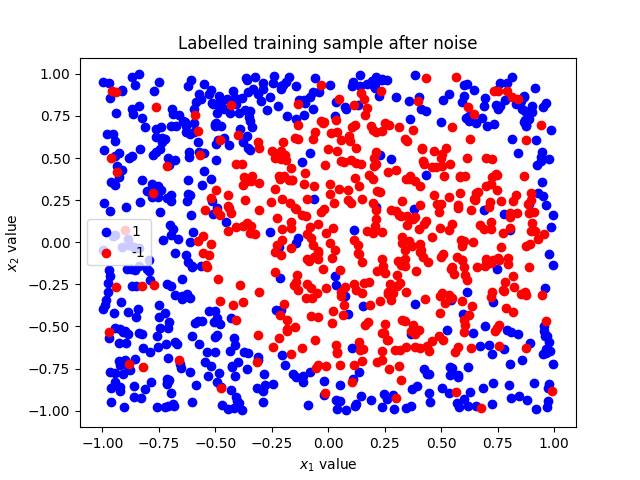
\includegraphics[width=\linewidth]{2_2_b_labelled_after_noise.png}
  

  \subsection{ Estimate the fitting error of $E_{in}$ using SGD}

  \subsubsection{Experiment c}
  Using $(1, x_1, x_2)$ as feature vector, fit a linear regression model to the generated datasets and estimate the weights w. Estimate the fitting error of Ein using Stochastic Gradient Descent (SGD).

  Having in mind the observation in the last subsection that the labels follow a circumference's equation with a bit of noise, a linear regression model it is not going to be the best approach.

  The experiment results are:
\begin{verbatim}
EXPERIMENT (c) 

	SGD, batch size 5
Ein:  0.9038395322567018

Evaluating output training data set
For w^T = [[ 0.05824863 -0.51637342  0.06313758]]
Input size:  1000
Bad negatives : 163
Bad positives : 212
Accuracy rate : 62.5 %
\end{verbatim}


Remember that the bad negatives are the points that the regression classify in negative but they are positives and the bad positives are the negative ones that are classify as a positives.

Finally the accuracy rate was the corrected classify data divided by the input size, so it is not a good model due to the fact that the accuracy rate is so close to a random one, that it would theoretically have a $50\%$ of accuracy rate.

A visual representation of the projection is


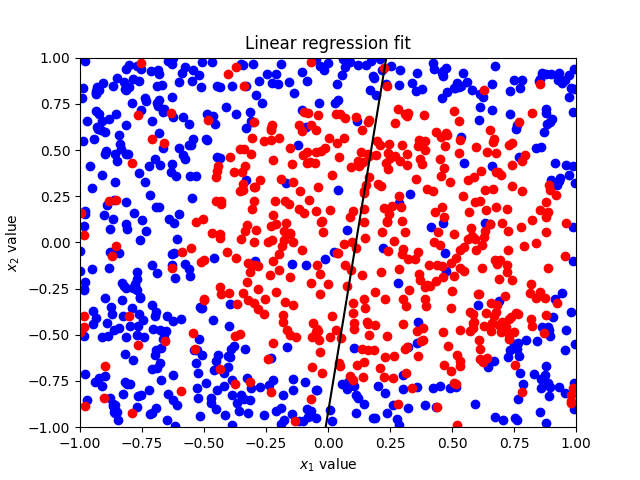
\includegraphics[width=\linewidth]{2_2_c_linear_regression.png}

\subsubsection{d) Repetition of the experiment}

In order to see that the last result was not hazaour we are going to repeat the experiment 1000 times, the result is:

\begin{verbatim}

 EXPERIMENT (d), lineal regression

The mean value of E_in in all 1000 experiments is: 0.9270571984798377
The mean value of E_out in all 1000 experiments is: 0.9330084274789892

\end{verbatim}


So as we can se the mean error is even worse hence, our linear regression is not a good one.

\subsubsection{e) Quadratic adjustment}

e) Assess how good you consider the fit with this linear model is according to the mean values obtained for Ein and Eout. Repeat the same previous experiment but using non-linear characteristics. Now, we will use the following feature vector: $\phi_2(x) =(1,x_1,x_2,x_1 x_2, x_1^2, x_2^2)$. Fit the new linear regression model and calculate the new vector of weights w. Calculate the average errors of Ein and Eout. Which model do you consider the most appropriate according to the average errors for Ein and Eout?



Now, instead of using a linear features vector, we are going to use a quadratic one

\begin{minted}{python}
  def quadraticFeatureVector(x_n):
        '''
        INPUT 
         xn = (x1,x2) vector of coordinates 
        
        '''
        return np.array([ 1,
                   x_n[0],
                   x_n[1],
                   x_n[0]*x_n[1],
                   x_n[0]* x_n[0],
                   x_n[1]* x_n[1]  ])

                 \end{minted}

                 We know that the function is a circumference with a 10\% of noise, so apriori we now that our target function is going to be

               
                 $$h(x,y) = (x-0.2)^2 + y^2 -0.6 = x^2 - 0.4x + 0.04 + y^2 - 0.6 = x^2 + y^2 - 0.4x - 0.56$$

                 What means that our target weight vector is goint to be

                 $$w_t = (-0.56, -0.4, 0,0,1,1)$$

                 Moreover due to the fact that we are introducing 10\% of noisy our accuracy level must be around $90\%$

                After $1000$ iterations we obtain:

 \begin{verbatim}
 SGD, batch size 5, number iterations 1000
Ein:  0.5724680127717665

Evaluating output training data set
For w^T = 
[[-0.67345368 -0.45209455 -0.0521589   0.07569398  0.92011803  1.23673771]]
Input size:  1000
Bad negatives : 94
Bad positives : 55
Accuracy rate : 85.1 %

\end{verbatim}

                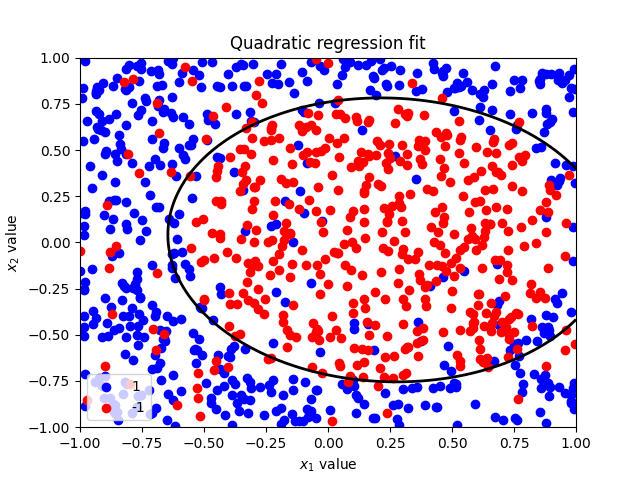
\includegraphics[width=\linewidth]{2_3_parabolle.png}

                
                
                The results are close to our first approach,
                
                but apriori, for $1000$ iterations they seen a bit bad.

                However if we analyse how the error, accuracy rate and $w$ are evoluting over $10, 50, 100, 200, 500, 700, 1000$ we clearly see that the error is improving, so the iterations were not enought.

                Something interesting is that the $700$ iterations have better accuracy rate than 1000, this is for the same reason we explained at exercise 1; we are minimazing the error, not the accuracy rate.    
       

 \begin{verbatim}

For one experiment:

 SGD, batch size 5, number iterations 10
Ein:  0.96683465968506

Evaluating output training data set
For w^T =
[[ 0.02353559 -0.04212481 -0.00067979  0.00785992  0.02654321  0.03756063]]
Input size:  1000
Bad negatives : 0
Bad positives : 474
Accuracy rate : 52.6 %

For one experiment:

 SGD, batch size 5, number iterations 50
Ein:  0.8964601273439083

Evaluating output training data set
For w^T =
 [[-0.00103819 -0.136871   -0.01033269  0.00363211  0.1056979   0.14178948]]
Input size:  1000
Bad negatives : 34
Bad positives : 266
Accuracy rate : 70.0 %

For one experiment:

 SGD, batch size 5, number iterations 100
Ein:  0.8337613668693657

Evaluating output training data set
For w^T = [[-0.04576936 -0.244725   -0.00396614  0.015827    0.19350407  0.24068118]]
Input size:  1000
Bad negatives : 64
Bad positives : 198
Accuracy rate : 73.8 %

For one experiment:

 SGD, batch size 5, number iterations 200
Ein:  0.751970586436338

Evaluating output training data set
For w^T = [[-0.16858105 -0.3725849  -0.01499836  0.02664101  0.30993404  0.4367047 ]]
Input size:  1000
Bad negatives : 93
Bad positives : 121
Accuracy rate : 78.6 %

For one experiment:

 SGD, batch size 5, number iterations 500
Ein:  0.6352766784644138

Evaluating output training data set
For w^T = 
[[-0.41975341 -0.46092311 -0.02902233  0.06514428  0.6286317   0.84761192]]
Input size:  1000
Bad negatives : 80
Bad positives : 72
Accuracy rate : 84.8 %

For one experiment:

 SGD, batch size 5, number iterations 700
Ein:  0.5997408279310205

Evaluating output training data set
For w^T = 
[[-0.53430804 -0.46110075 -0.0464511   0.06892706  0.76915291  1.04094009]]
Input size:  1000
Bad negatives : 78
Bad positives : 63
Accuracy rate : 85.9 %

For one experiment:

 SGD, batch size 5, number iterations 1000
Ein:  0.5724680127717665

Evaluating output training data set
For w^T = 
[[-0.67345368 -0.45209455 -0.0521589   0.07569398  0.92011803  1.23673771]]
Input size:  1000
Bad negatives : 94
Bad positives : 55
Accuracy rate : 85.1 %

\end{verbatim}


\subsubsection{Mean error and conclusion}


In order to see the last result was not hazaour we are going to repeat the experiment 1000 times, the result is:


\begin{verbatim}
The mean value of E_in in all 1000 experiments is: 0.600107053636983
The mean value of E_out in all 1000 experiments is: 0.6058641910896161
\end{verbatim}

More or less the error is the same, so we can trust that a good adjustment is a quadratic one.

Something which we have known a priori, because we knew our target vector (something that in real life does not happen).

